\documentclass{tufte-handout}

\title{Utility Theory and the Representation of Preference}

\author[Nathaniel Forde]{Nathaniel Forde}

%\date{28 March 2010} % without \date command, current date is supplied

%\geometry{showframe} % display margins for debugging page layout

\usepackage{graphicx} % allow embedded images
  \setkeys{Gin}{width=\linewidth,totalheight=\textheight,keepaspectratio}
  \graphicspath{{graphics/}} % set of paths to search for images
\usepackage{amsmath}  % extended mathematics
\usepackage{booktabs} % book-quality tables
\usepackage{units}    % non-stacked fractions and better unit spacing
\usepackage{multicol} % multiple column layout facilities
\usepackage{lipsum}   % filler text
\usepackage{fancyvrb} % extended verbatim environments
  \fvset{fontsize=\normalsize}% default font size for fancy-verbatim environments
\usepackage{minted}

% Standardize command font styles and environments
\newcommand{\doccmd}[1]{\texttt{\textbackslash#1}}% command name -- adds backslash automatically
\newcommand{\docopt}[1]{\ensuremath{\langle}\textrm{\textit{#1}}\ensuremath{\rangle}}% optional command argument
\newcommand{\docarg}[1]{\textrm{\textit{#1}}}% (required) command argument
\newcommand{\docenv}[1]{\textsf{#1}}% environment name
\newcommand{\docpkg}[1]{\texttt{#1}}% package name
\newcommand{\doccls}[1]{\texttt{#1}}% document class name
\newcommand{\docclsopt}[1]{\texttt{#1}}% document class option name
\newenvironment{docspec}{\begin{quote}\noindent}{\end{quote}}% command specification environment

\begin{document}

\maketitle% this prints the handout title, author, and date

\begin{abstract}
\noindent
This article continues the investigation of the expected utility model of rational choice. We begin by examining how preference relates to utility, before continuing to the representation theorems which formalise the connection. Will we see that the nature of these theorems, coupled with the indeterminacy of statistical inference is a brittle foundation for predictive economic models of consumer choice.
\end{abstract}


\section{From Utility to Indifference}
Too much of a good thing often tends to the bad. So we dabble, sample and share. In pursuit of variety we swap our goods, shunning stale options in favour of the novel exchange.  For a given good we can differ in our appetites but it's relatively straightforward to find the point where one more donut is one too many. While it can be a bit unclear how we should measure utility, once we've decided on a metric the mathematical characteristics are meaningful. We can infer aspects of your attitudes towards acquisition and enthusiasm for donuts. In most cases we're interested not just in your pursuit of pastries, but how you'd be willing to trade for those pastries. 

\begin{marginfigure}
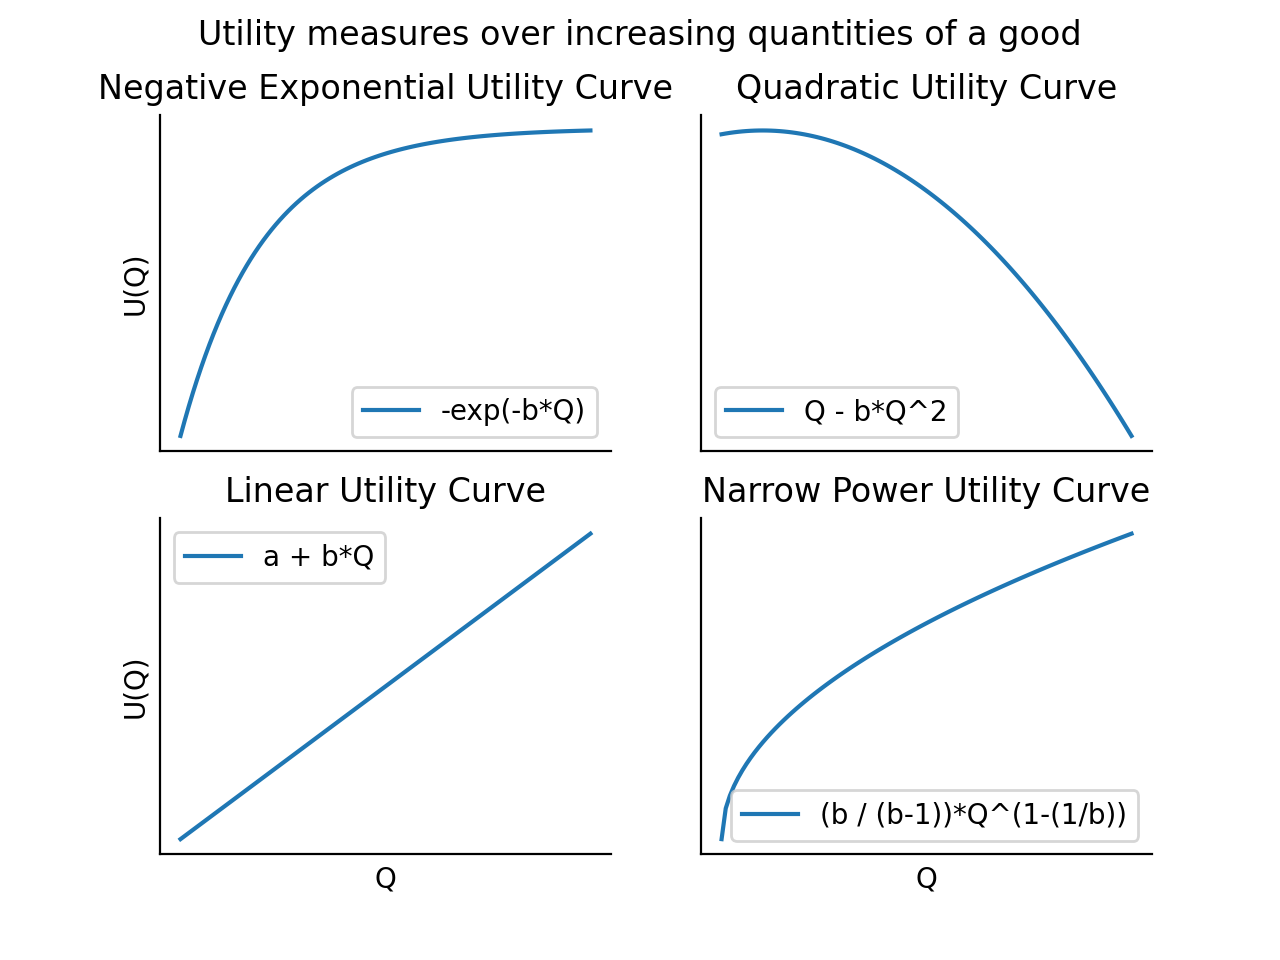
\includegraphics[width=3in]{Plots/utility_in_1_dimension.png}
\caption{Consumer attitudes with differently satisfied appetites for a good}
\includegraphics[width=3in]{Plots/derivatives_of_utility.png}
\caption{The Rates of Change of personal Utility}
\end{marginfigure} 

The possibility of coordinated compromise lies at the core of maximising subjective utility. We seek competitive advantage for our own produce to balance the cost owed to the skills of others. At the limit some trades do not admit any mixture of goods. Not all babies can be cut in half. On the other side of the spectrum, there are some things which we'd give everything. In most cases though a consumer will try to optimise their bundle of goods over an entire marketplace, preserving enough on one key good; money, to remain liquid. 

$$ u(\overrightarrow{g}) = f(g_{0}, g_{1} ... g_{n}) $$

There are number of ways we can specify a utility function, but a typical example is the Cobb-Douglas function. 

$$ u(\overrightarrow{g}) = g_{0}^{\alpha_{0}}g_{1}^{\alpha_{1}} ... g_{n}^{\alpha_{n}}$$

\begin{marginfigure}
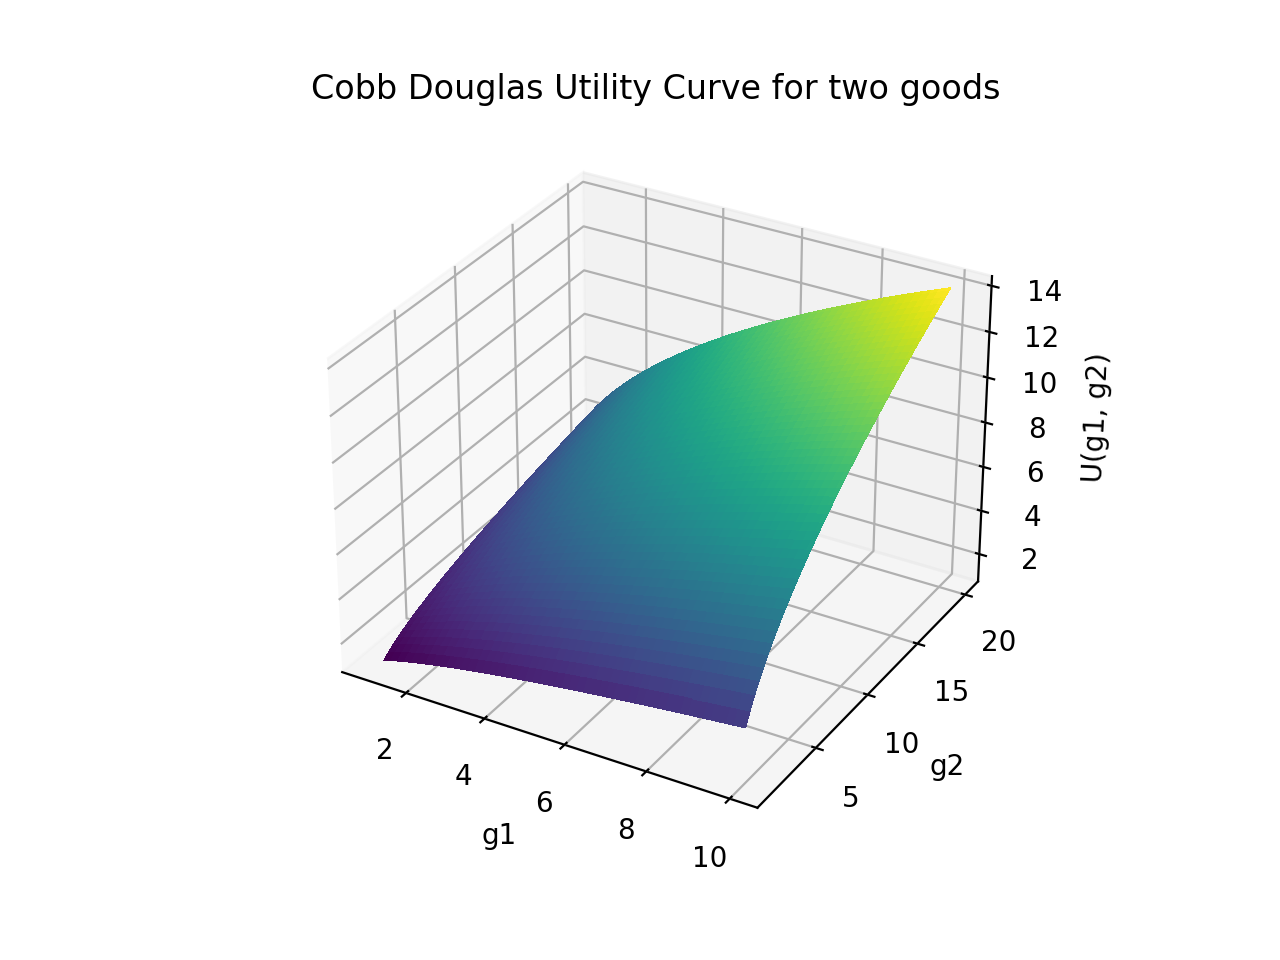
\includegraphics[width=3.2in, height=5.in]{Plots/cobb_douglas_utility.png}
\caption{A consumers utility curve for combinations of two goods}
\end{marginfigure} 

Then taking the case of two goods $g1, g2$ we can determine an indifference curve where you would be willing to exchange quantities of $g1$ for an agreeable amount of $g2$.  Set 
$$u(\overrightarrow{g}) = k =  g_{1}^{\frac{1}{2}}g_{2}^{\frac{1}{2}} = (g_{1}g_{2})^{\frac{1}{2}}  = \sqrt{g_{1}g_{2}}$$
$$ \Rightarrow k^{2} = g_{1}g_{2} \Rightarrow \frac{k^{2}}{g_{2}} = g_{1}$$

Using this we can plot the quantities of fair exchange based on the mutivariate utility function. This is not to say that these curves represent an actual or objective fair price, just that when measured in terms of utility these are mappings of quantities of good we would be happy to exchange.

\begin{marginfigure}
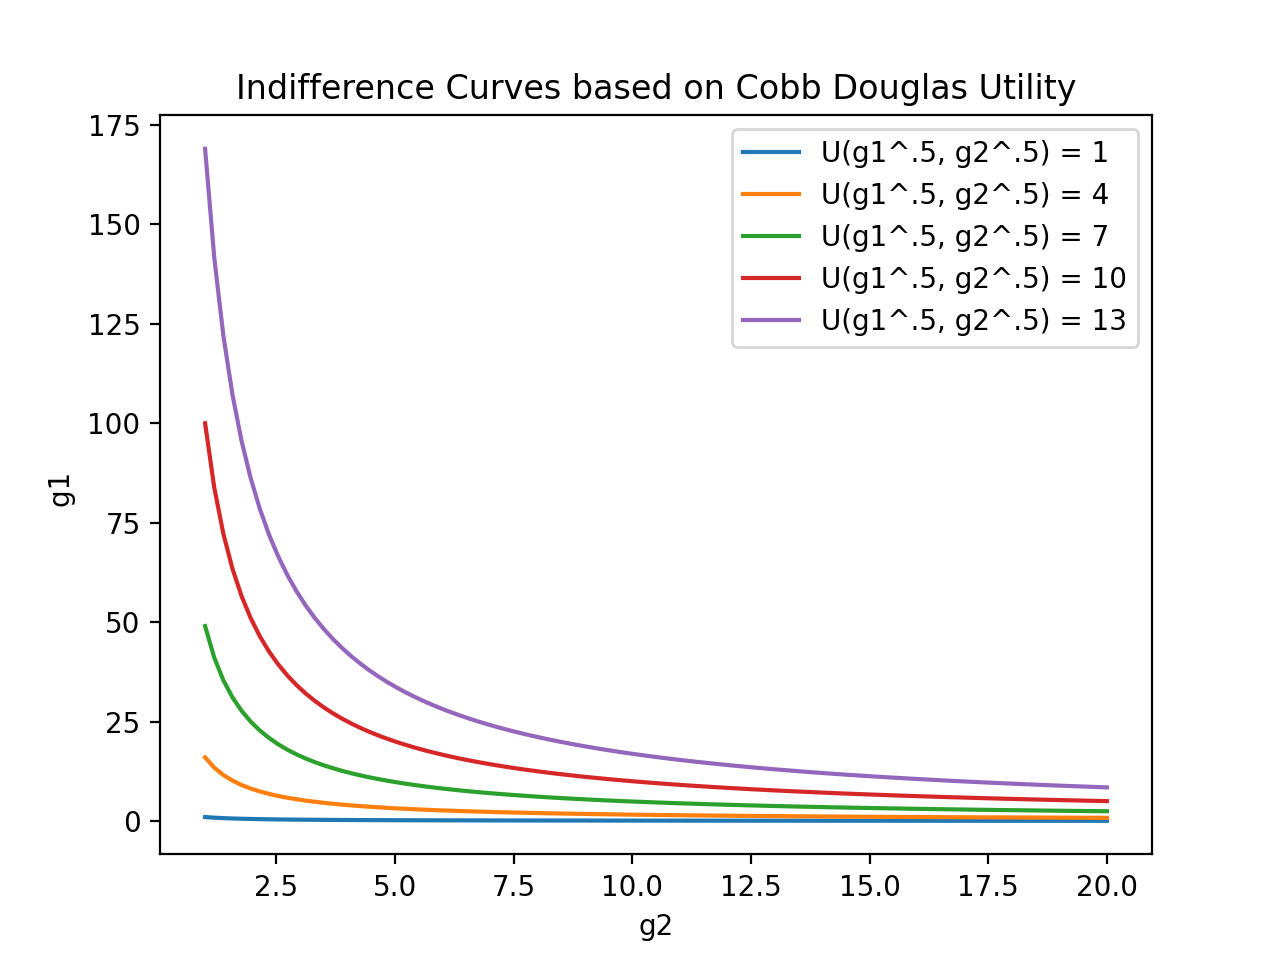
\includegraphics[width=3in, height=5.in]{Plots/indifference_curves.png}
\end{marginfigure}

Our view of a fair price is encoded in our utility theory. It's at this point when economics is said to verge on empirical science. If we can model your preferences as a utility function characteristic of some general attitude toward acquisition, we might also hope to able to predict future trades.  

\begin{minted}{Python}

def function(x):
	efwfewf

\end{minted}

\bibliography{sample-handout}
\bibliographystyle{plainnat}



\end{document}
